%%%%%%%%%%%%%%%%%%%%%%%%%%%%%%%%%%%%%%%%%%%%%%%%%%%%%%%%%%%%%%%%%%%%%%%%%%%%%%%%
%%%%%%%%%%%%%%%%%%%%%%%%%%%%%%%%%%%%%%%%%%%%%%%%%%%%%%%%%%%%%%%%%%%%%%%%%%%%%%%%
%%%%%%%%%%%%%%%%%%%%%%%%%%%%%%%%%%%%%%%%%%%%%%%%%%%%%%%%%%%%%%%%%%%%%%%%%%%%%%%%
%%%%%%%%%%%%%%%%%%%%%%%%%%%%%%%%%%%%%%%%%%%%%%%%%%%%%%%%%%%%%%%%%%%%%%%%%%%%%%%%
\chapter{Transformée de Laplace inverse~\label{annexe-invL}}
%%%%%%%%%%%%%%%%%%%%%%%%%%%%%%%%%%%%%%%%%%%%%%%%%%%%%%%%%%%%%%%%%%%%%%%%%%%%%%%%
%%%%%%%%%%%%%%%%%%%%%%%%%%%%%%%%%%%%%%%%%%%%%%%%%%%%%%%%%%%%%%%%%%%%%%%%%%%%%%%%
%%%%%%%%%%%%%%%%%%%%%%%%%%%%%%%%%%%%%%%%%%%%%%%%%%%%%%%%%%%%%%%%%%%%%%%%%%%%%%%%
%%%%%%%%%%%%%%%%%%%%%%%%%%%%%%%%%%%%%%%%%%%%%%%%%%%%%%%%%%%%%%%%%%%%%%%%%%%%%%%%

%%%%%%%%%%%%%%%%%%%%%%%%%%%%%%%%%%%%%%%%%%%%%%%%%%%%%%%%%%%%%%%%%%%%%%%%%%%%%%%%
%%%%%%%%%%%%%%%%%%%%%%%%%%%%%%%%%%%%%%%%%%%%%%%%%%%%%%%%%%%%%%%%%%%%%%%%%%%%%%%%
%%%%%%%%%%%%%%%%%%%%%%%%%%%%%%%%%%%%%%%%%%%%%%%%%%%%%%%%%%%%%%%%%%%%%%%%%%%%%%%%
\section{Contexte}
%%%%%%%%%%%%%%%%%%%%%%%%%%%%%%%%%%%%%%%%%%%%%%%%%%%%%%%%%%%%%%%%%%%%%%%%%%%%%%%%
%%%%%%%%%%%%%%%%%%%%%%%%%%%%%%%%%%%%%%%%%%%%%%%%%%%%%%%%%%%%%%%%%%%%%%%%%%%%%%%%
%%%%%%%%%%%%%%%%%%%%%%%%%%%%%%%%%%%%%%%%%%%%%%%%%%%%%%%%%%%%%%%%%%%%%%%%%%%%%%%%
Il existe une forme analytique de la transformée inverse basée sur
la formule de Mellin-Fourier\cite{Ostertag}:
\[
s(t)=\laplacei{S(p)}=\int_{c-j\infty}^{c+j\infty} e^{pt}S(p)\dd{p}
\]
Cette inversion se fait donc par le biais d'une intégrale dans le plan
complexe. Cette intégrale n'ayant pas de forme analytique, il n'est possible 
d'approcher une solution qu'à l'aide d'outils numérique. 
Dans cette annnexe, nous discuterons deux implémentations en python de 
deux de ces algorithmes : 
l'algorithme de Gaver-Stehfest et l'algorithme fixe de Talbot comme présentés
par Abate et al.~\cite{abate2004,abate2006,frwiki:200676411}.
Avant de tester ces méthodes sur les systèmes linéaires, nous l'appliquerons
à l'inversion de Laplace :  
\[
    te^{-t}=\laplacei{\dfrac{1}{(p+1)^2}},
\]
dont on connait la forme analytique exacte.
Il faut noter que les méthodes et algorithmes présentés ici dépendent 
largement de la précision machine accessible pour le calcul en virgule flottante.
L'usage de librairie en précision arbitraire comme \texttt{mpmath} peut être 
nécessaire pour obtenir des résultats de meilleure précision. Il est également
connu que toutes les méthodes d'inversion numérique présente des problèmes
aux temps longs lorsque la fonction à inverser présente des pôles ce qui 
est très largement le cas des SLCI.
%%%%%%%%%%%%%%%%%%%%%%%%%%%%%%%%%%%%%%%%%%%%%%%%%%%%%%%%%%%%%%%%%%%%%%%%%%%%%%%%
%%%%%%%%%%%%%%%%%%%%%%%%%%%%%%%%%%%%%%%%%%%%%%%%%%%%%%%%%%%%%%%%%%%%%%%%%%%%%%%%
%%%%%%%%%%%%%%%%%%%%%%%%%%%%%%%%%%%%%%%%%%%%%%%%%%%%%%%%%%%%%%%%%%%%%%%%%%%%%%%%
\section{Algorithme de Gaver-Stehfest}
%%%%%%%%%%%%%%%%%%%%%%%%%%%%%%%%%%%%%%%%%%%%%%%%%%%%%%%%%%%%%%%%%%%%%%%%%%%%%%%%
%%%%%%%%%%%%%%%%%%%%%%%%%%%%%%%%%%%%%%%%%%%%%%%%%%%%%%%%%%%%%%%%%%%%%%%%%%%%%%%%
%%%%%%%%%%%%%%%%%%%%%%%%%%%%%%%%%%%%%%%%%%%%%%%%%%%%%%%%%%%%%%%%%%%%%%%%%%%%%%%%
La transformée inverse par la méthode de Gaver-Stehfest est donné par 
(relation adaptée de l'équation (31) de~\cite{abate2006}) :
\[
f(t)=\dfrac{\ln{2}}{t}\sum_{k=1}^{2M}\zeta_kF\left(\dfrac{k\ln{2}}{t}\right)
\]
où l'on note $f(t)$ la fonction inverse de $F(p)$ et les $\zeta_k$ sont
donnés par la relation (32) de~\cite{abate2006} c'est à dire :
\[
\zeta_k = (-1)^{M+k} \sum_{j=\lfloor(k+1)/2\rfloor}^{\min{(k,M)}} 
\dfrac{j^{M+1}}{M!}\begin{pmatrix} M\\j  \end{pmatrix}
                   \begin{pmatrix} 2j\\j \end{pmatrix}
                   \begin{pmatrix} j\\k-j\end{pmatrix}
\]
avec $\lfloor x \rfloor$ le plus grand entier inférieur ou égal à $x$. Il 
nous faudra définir les coefficients binomiaux et les $\zeta_k$ avec les
deux fonctions suivantes :
\clearpage
%-------------------------------------------------------------------------------
\inputminted{python}{codes/python/coeff_bin-annexe_invL.py}
%-------------------------------------------------------------------------------
%-------------------------------------------------------------------------------
\inputminted{python}{codes/python/zeta-annexe_invL.py}
%-------------------------------------------------------------------------------
\clearpage
%-------------------------------------------------------------------------------
\inputminted{python}{codes/python/gaver_stehfest-annexe_invL.py}
%-------------------------------------------------------------------------------
La fonction \texttt{gaver\_stehfest} prend en paramètres 
le temps \texttt{t} et une fonction \texttt{f} représentant la fonction inverse 
$F(p)$.
%%%%%%%%%%%%%%%%%%%%%%%%%%%%%%%%%%%%%%%%%%%%%%%%%%%%%%%%%%%%%%%%%%%%%%%%%%%%%%%%
%%%%%%%%%%%%%%%%%%%%%%%%%%%%%%%%%%%%%%%%%%%%%%%%%%%%%%%%%%%%%%%%%%%%%%%%%%%%%%%%
\subsection*{Test de la méthode}
%%%%%%%%%%%%%%%%%%%%%%%%%%%%%%%%%%%%%%%%%%%%%%%%%%%%%%%%%%%%%%%%%%%%%%%%%%%%%%%%
%%%%%%%%%%%%%%%%%%%%%%%%%%%%%%%%%%%%%%%%%%%%%%%%%%%%%%%%%%%%%%%%%%%%%%%%%%%%%%%%
Soit la transformée de Laplace inverse connue :
\[
    te^{-t}=\laplacei{\dfrac{1}{(p+1)^2}}
\]
Nous cherchons à déterminer numériquement la transformée inverse 
pour différentes valeurs de $t\in[10^{-1},10^3]$  
\begin{minted}{python}
ft=lambda t : t*exp(-t)
fp=lambda p : 1/(p+1)**2
t=np.logspace(-1,3,256)
f_gaver_stehfest=np.array([gaver_stehfest(tk,fp,20) for tk in t])
f_analytic=np.array([ft(tk) for tk in t])
\end{minted}
Nous traçons ci-dessous la différence relative entre ces deux fonctions.
%-------------------------------------------------------------------------------
\begin{figure}[!b]
    \centering
    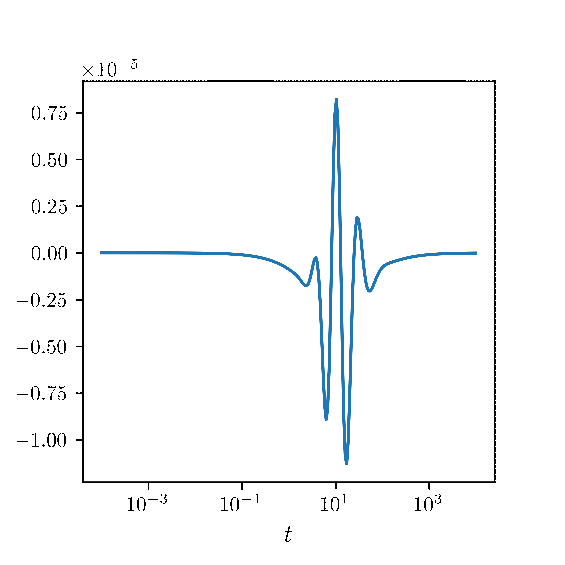
\includegraphics[width=0.4\linewidth]{erreur_gaver-stehfest.eps}
    \caption{Erreur relative de l'algorithme de Gaver-Stehfest} 
\end{figure}
%-------------------------------------------------------------------------------
\clearpage
%%%%%%%%%%%%%%%%%%%%%%%%%%%%%%%%%%%%%%%%%%%%%%%%%%%%%%%%%%%%%%%%%%%%%%%%%%%%%%%%
%%%%%%%%%%%%%%%%%%%%%%%%%%%%%%%%%%%%%%%%%%%%%%%%%%%%%%%%%%%%%%%%%%%%%%%%%%%%%%%%
%%%%%%%%%%%%%%%%%%%%%%%%%%%%%%%%%%%%%%%%%%%%%%%%%%%%%%%%%%%%%%%%%%%%%%%%%%%%%%%%
\section{Algorithme fixe de Talbot}
%%%%%%%%%%%%%%%%%%%%%%%%%%%%%%%%%%%%%%%%%%%%%%%%%%%%%%%%%%%%%%%%%%%%%%%%%%%%%%%%
%%%%%%%%%%%%%%%%%%%%%%%%%%%%%%%%%%%%%%%%%%%%%%%%%%%%%%%%%%%%%%%%%%%%%%%%%%%%%%%%
%%%%%%%%%%%%%%%%%%%%%%%%%%%%%%%%%%%%%%%%%%%%%%%%%%%%%%%%%%%%%%%%%%%%%%%%%%%%%%%%
On souhaite se donner la relation (18) de~\cite{abate2004} 
qui se présente sous la forme :
\[
f(t) = \dfrac{r}{M} 
\left\{ 
    \dfrac{1}{2} F(r) e^{rt}+ \sum_{k=1}^{M-1} 
    \textrm{Re}\left[ e^{ts(\theta_k)} F(s(\theta_k)) (1+i\sigma(\theta_k))\right]
\right\}
\]
avec $\theta_k=\frac{k\pi}{M}$, et les relations (19), (16) et (11) de [3] 
sont nécessaires pour implémenter la méthode à savoir 
$r=\frac{2M}{5t}$,$\sigma(\theta)=\theta+(\theta\cot\theta-1)\cot\theta$,
$s(\theta)=r\theta(\cot\theta+i)$.
\inputminted{python}{codes/python/talbot-annexe_invL.py}
%%%%%%%%%%%%%%%%%%%%%%%%%%%%%%%%%%%%%%%%%%%%%%%%%%%%%%%%%%%%%%%%%%%%%%%%%%%%%%%%
%%%%%%%%%%%%%%%%%%%%%%%%%%%%%%%%%%%%%%%%%%%%%%%%%%%%%%%%%%%%%%%%%%%%%%%%%%%%%%%%
\subsection*{Test de la méthode}
%%%%%%%%%%%%%%%%%%%%%%%%%%%%%%%%%%%%%%%%%%%%%%%%%%%%%%%%%%%%%%%%%%%%%%%%%%%%%%%%
%%%%%%%%%%%%%%%%%%%%%%%%%%%%%%%%%%%%%%%%%%%%%%%%%%%%%%%%%%%%%%%%%%%%%%%%%%%%%%%%
Nous cherchons à nouveau à reproduire la transformée de Laplace inverse :
\[
    te^{-t}=\laplacei{\dfrac{1}{(p+1)^2}}
\]
La différence relative entre l'algorithme fixe de Talbot et le résultat exact 
est donnée ci-dessous
%-------------------------------------------------------------------------------
\begin{figure}[!b]
    \centering
    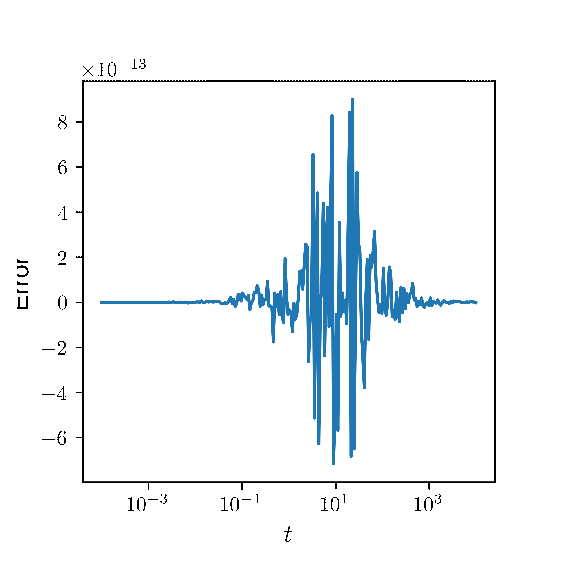
\includegraphics[width=0.4\linewidth]{erreur_talbot.eps}
    \caption{Erreur relative de l'algorithme fixe de Talbot} 
\end{figure}
%-------------------------------------------------------------------------------
\clearpage
%%%%%%%%%%%%%%%%%%%%%%%%%%%%%%%%%%%%%%%%%%%%%%%%%%%%%%%%%%%%%%%%%%%%%%%%%%%%%%%%
%%%%%%%%%%%%%%%%%%%%%%%%%%%%%%%%%%%%%%%%%%%%%%%%%%%%%%%%%%%%%%%%%%%%%%%%%%%%%%%%
%%%%%%%%%%%%%%%%%%%%%%%%%%%%%%%%%%%%%%%%%%%%%%%%%%%%%%%%%%%%%%%%%%%%%%%%%%%%%%%%
\section{Applications aux SLCI}
%%%%%%%%%%%%%%%%%%%%%%%%%%%%%%%%%%%%%%%%%%%%%%%%%%%%%%%%%%%%%%%%%%%%%%%%%%%%%%%%
%%%%%%%%%%%%%%%%%%%%%%%%%%%%%%%%%%%%%%%%%%%%%%%%%%%%%%%%%%%%%%%%%%%%%%%%%%%%%%%%
%%%%%%%%%%%%%%%%%%%%%%%%%%%%%%%%%%%%%%%%%%%%%%%%%%%%%%%%%%%%%%%%%%%%%%%%%%%%%%%%
Nous souhaitons appliquer les deux approches aux calculs de la réponse 
indicielle d'un système du premier et du second ordre. 
Nous utiliserons les relations exactes obtenues au chapitre~\cref{chap-model} 
pour comparer les résultats obtenus.

%%%%%%%%%%%%%%%%%%%%%%%%%%%%%%%%%%%%%%%%%%%%%%%%%%%%%%%%%%%%%%%%%%%%%%%%%%%%%%%%
%%%%%%%%%%%%%%%%%%%%%%%%%%%%%%%%%%%%%%%%%%%%%%%%%%%%%%%%%%%%%%%%%%%%%%%%%%%%%%%%
\subsection*{Système du 1er ordre}
%%%%%%%%%%%%%%%%%%%%%%%%%%%%%%%%%%%%%%%%%%%%%%%%%%%%%%%%%%%%%%%%%%%%%%%%%%%%%%%%
%%%%%%%%%%%%%%%%%%%%%%%%%%%%%%%%%%%%%%%%%%%%%%%%%%%%%%%%%%%%%%%%%%%%%%%%%%%%%%%%
%La fonction python ci-dessous permet de calculer la réponse indicielle au temps
%$t$ d'un système du premier ordre pour des paramètres $K$ et $\tau$ données.
%-------------------------------------------------------------------------------
%\inputminted{python}{codes/python/1er_ordre-annexe_invL.py}
%-------------------------------------------------------------------------------
%-------------------------------------------------------------------------------
\begin{figure}[!b]
    \centering
    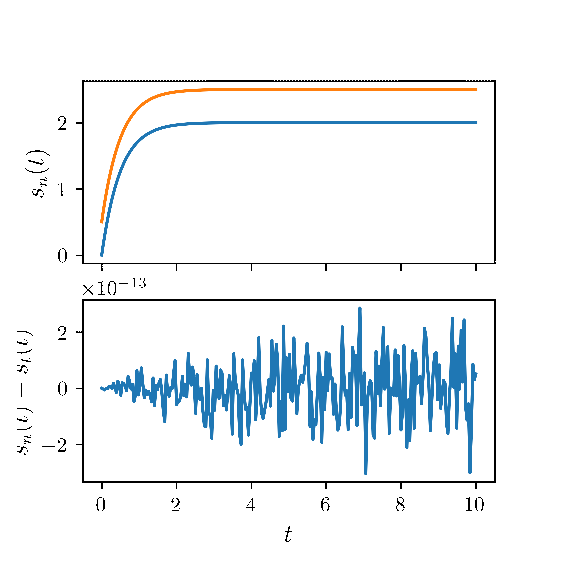
\includegraphics[width=0.9\linewidth]{1er_ordre_talbot.eps}
    \caption[1erOrdreInvL]{
    \textbf{(en haut)} Réponses temporelles d'un système du premier ordre 
    calculées à l'aide de (bleu) l'algorithme 
    fixe de Talbot et (orange) la méthode de Gaver-Stehfest. Les deux réponses
    sont légerement décaler pour permettre la comparaison

    \textbf{(en bas)} Différence
    relative de chacunes des deux approches avec la réponse temporelle exacte calculée
    avec la fonction \texttt{premier\_ordre}.~\label{fig-1erOrdreInvL}}
\end{figure}
%-------------------------------------------------------------------------------
\clearpage
%%%%%%%%%%%%%%%%%%%%%%%%%%%%%%%%%%%%%%%%%%%%%%%%%%%%%%%%%%%%%%%%%%%%%%%%%%%%%%%%
%%%%%%%%%%%%%%%%%%%%%%%%%%%%%%%%%%%%%%%%%%%%%%%%%%%%%%%%%%%%%%%%%%%%%%%%%%%%%%%%
\subsection*{Système du 2nd ordre}
%%%%%%%%%%%%%%%%%%%%%%%%%%%%%%%%%%%%%%%%%%%%%%%%%%%%%%%%%%%%%%%%%%%%%%%%%%%%%%%%
%%%%%%%%%%%%%%%%%%%%%%%%%%%%%%%%%%%%%%%%%%%%%%%%%%%%%%%%%%%%%%%%%%%%%%%%%%%%%%%%

%-------------------------------------------------------------------------------
%\inputminted{python}{codes/python/2nd_ordre-annexe_invL.py}
%-------------------------------------------------------------------------------
%-------------------------------------------------------------------------------
\begin{figure}[!b]
    \centering
    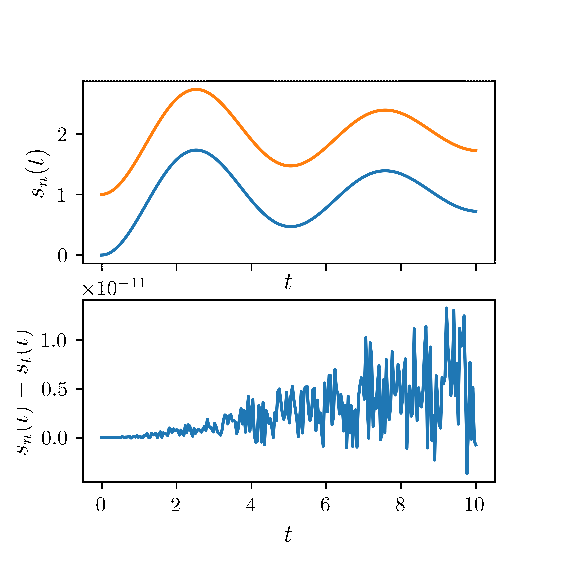
\includegraphics[width=0.9\linewidth]{2nd_ordre_talbot.eps}
    \caption{Même présentation que~\cref{fig-1erOrdreInvL} dans le cas d'un système
    du second ordre}
\end{figure}
%-------------------------------------------------------------------------------
%%%%%%%%%%%%%%%%%%%%%%%%%%%%%%%%%%%%%%%%%%%%%%%%%%%%%%%%%%%%%%%%%%%%%%%%%%%%%%%%
%%%%%%%%%%%%%%%%%%%%%%%%%%%%%%%%%%%%%%%%%%%%%%%%%%%%%%%%%%%%%%%%%%%%%%%%%%%%%%%%
%%%%%%%%%%%%%%%%%%%%%%%%%%%%%%%%%%%%%%%%%%%%%%%%%%%%%%%%%%%%%%%%%%%%%%%%%%%%%%%%
%%%%%%%%%%%%%%%%%%%%%%%%%%%%%%%%%%%%%%%%%%%%%%%%%%%%%%%%%%%%%%%%%%%%%%%%%%%%%%%%
%annexe_invL.tex
